% 经典力学
% 经典力学|牛顿力学|刚体|流体|分析力学|相对论

\pentry{物理理论\upref{MecThe}}

\subsection{经典力学}
经典力学描述的是若干(宏观低速)的粒子(就是高中所讲的\textbf{质点})受若干力以后的运动情况. 牛顿三定律\upref{New3}可以作为经典力学的\textbf{公设}. 公设在这里指的是某个理论体系(例如经典力学)内的基本假设. 由这些假设可以推导出理论体系中的所有推论, 但其本身却无法被推导而来\footnote{“无法被推导” 是在这个理论内部而言的. 一个理论的基本假设可以由更高级, 使用范围更广的理论的基本假设推导出来. 例如牛顿第二定律可以由狭义相对论或量子力学的基本假设推导而来.}, 只能通过实验证明. 我们可以将牛顿三定律想象成一个懂经典力学的电脑, 只需输入初始时刻所有粒子的状态(位置和速度/动量),以及每个粒子的受力/势能函数,就可以得到接下来每个粒子的运动方式(位置关于时间的函数). 我们在研究某个问题时,往往把讨论范围内的粒子叫做\textbf{系统}.

例如我们要研究太阳系中行星的运动, 就往往把这些行星看作是粒子(质点), 这是因为比起他们的距离来, 他们本身的大小可以忽略不计\footnote{在物理中, 我们经常使用这种手段简化问题, 并将其称为\textbf{近似}}. 我们只要知道某时刻(初始时刻)它们的位置和动量(在大学物理中, 你会发现我们更多地使用动量而不是速度, 在已知质量的情况下, 它们所包含的信息是一样的, 即一一对应), 将它们输入“牛顿三定律” 这台电脑中, 就可以得到接下来所有天体的运动情况, 即任意时刻任意粒子的位置和动量.

\subsection{刚体和流体}
质点的模型忽略了物体的实际大小, 如果要考虑一个大小不可忽略的物体的转动, 以及若干个大小不可忽略的物体之间的相互作用该怎么办? 事实上, 这些物体也是由原子和分子构成的\footnote{经典力学不能准确描述原子的结构和运动, 要使用量子力学, 但我们这里讨论的是组成物体后的宏观运动, 所以即使用经典力学来描述原子得到的宏观运动也是正确的}. 在固体中, 原子之间的作用力使它们相对位置较难改变, 例如可以想象每个原子和与它相邻的原子都以较硬的弹簧相连. 所以, 我们同样可以把这些物体看作是由质点组成得. 这样, 我们就可以用质点的力学来描述有形状有质量分布的物体了. 在力学中我们经常使用一种理想模型叫做\textbf{刚体}, 即假设物体中连接这些质点的弹簧的劲度系数为无限大, 或者把他们看成不可伸缩的棍子. 所以如果我们近似认为一个物体无限硬, 忽略其自身的形变, 我们就可以用刚体的模型来描述它.

另一种物质的形态,液体, 同样可以用理想化的力学模型来描述, 我们把它叫做\textbf{流体}, 流体力学是力学中十分重要的分支, 轮船,高铁,飞机和火箭的设计都要使用它.

\subsection{受力决定运动}
经典力学中最简单的一类问题是: 已知初始时刻若干粒子的运动状态, 以及接下来每一个粒子的受力. 以直线运动为例, $F$ 随\textbf{时间} $t$ 的变化(即函数 $F(t)$). 根据牛顿第二定律, 可以求出每个粒子任意时刻的加速度 $a$(正比于 $F$), 进而求出速度 $v$ 随时间的变化, 也就是求“加速度—时间” 曲线下面在某段时间的面积(这在数学上叫做\textbf{定积分}). 有了速度随时间的变化, 我们又可以通过面积求位置随时间的变化(同样是定积分, 求“ 速度—时间” 曲线下面的面积). 例如我们知道一个沿直线运动的粒子受一个恒力(例如自由落体), 它的加速度是恒定的, 这个过程如\autoref{CM0_fig1}. 这种方法适用于任何形状的 $F(t)$ 曲线.

\begin{figure}[ht]
\centering
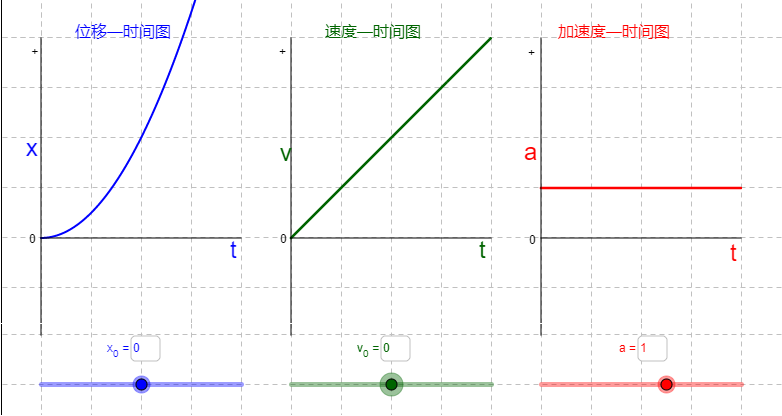
\includegraphics[width=14cm]{./figures/CM0_1.png}
\caption{匀加速直线运动(见 “\href{http://wuli.wiki/apps/consta.html}{互动演示}” 页面), 加速度曲线下方从 $0$ 到 $t$ 的面积是速度, 速度曲线下方从 $0$ 到 $t$ 的面积是位移} \label{CM0_fig1}
\end{figure}

\subsubsection{简谐振子}
为了方便下文举例, 我们先来介绍力学中的一个经典模型即\textbf{简谐振子}. 假设无摩擦的光滑水平直轨道上有一根质量不计的弹簧一端固定不动, 而另一端上固定了一个质点. 如果给这个质点一个初速度或初位移, 那么它将会沿着轨道往复运动, 我们把这种运动叫做\textbf{简谐运动}. 顺带一提, 我们以后会看到位置关于时间的函数恰好是 $\cos(\omega t)$, $\omega$ 是\textbf{角频率}, 代表振动的快慢.

\begin{figure}[ht]
\centering
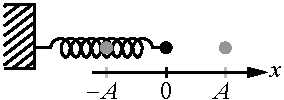
\includegraphics[width=6cm]{./figures/CM0_2.pdf}
\caption{简谐振子} \label{CM0_fig2}
\end{figure}

\subsection{更困难的问题}
事实上我们很少会遇到 “已知每个质点的 $F(t)$” 这么简单的条件. 即使在简谐振子这样简单的模型中, 我们也不可能事先就知道质点受力关于时间的变化情况. 因为受力分析得到的是力\textbf{关于位置}的变化($F(x) = -k x$, $k$ 是劲度系数), 而粒子的位置变化(函数 $x(t)$)又取决于受力. 这样一来, 我们就没有办法像上面一样直接用定积分来解决这个问题了.

为了解决这样的问题, 我们需要使用\textbf{微分方程}. 但现在我们可以用以下的简单思路进行一个近似的数值计算: 例如在简谐振子的模型中, 假设质点初始时刻处于弹簧的平衡位置 $x = 0$(受力为零)并具有一个初速度 $v_0$, 在很小一段时间 $\Delta t$ 内, 由于 $x$ 仍然很小, 我们可以继续认为质点不受力, 做匀速运动. 这样当它移动到 $x = v\Delta t$ 时, 我们重新计算它的受力得到 $F = -kx = x v \Delta t$, 然后假设在下一段很短的时间 $\Delta t$ 内仍然假设质点受力不变, 计算出位置和速度的变化. 如此循环, 就可以数值计算出 $x(t)$ 的一系列散点, 连起来就得到了位移—时间曲线. 当 $\Delta t$ 取得越小, 这种近似就越精确.

\subsection{分析力学}
分析力学的数学形式比牛顿定律复杂, 但和牛顿力学是等效的, 即任何分析力学计算的问题用牛顿定律同样能计算并得到完全相同的结果,反之亦然. 分析力学常见的形式有两种,一种是拉格朗日力学,使用拉格朗日方程,另一种叫哈密顿力学,使用哈密顿方程. 量子力学就是在哈密顿力学的基础上建立起来的,其重要性可见一斑.% (未完成:提一下位置和动量的重要性,广义坐标和广义动量)

相比与牛顿力学,分析力学的优势主要有两点. 一是当计算的系统越来越复杂的时候(例如蒸汽机等复杂的机械结构)分析力学一般能更快捷地列出微分方程组, 而牛顿力学所需要的受力分析会变得非常复杂. 另一方面, 分析力学能使我们站在更高的高度看问题(例如可以分析出系统中的守恒量).

为什么复杂的数学形式反而在一些情况下使列方程变得简单呢? 如果把牛顿定律比作电脑, 那么分析力学就相当于一个更智能的电脑, 对于系统中的某些物体, 无需告诉电脑它的受力, 只需告诉电脑它物体之间的运动的约束即可. 约束简单来说就是怎样的运动是不可能的:例如单摆中的质点就“不可能”沿着绳的方向运动,两个咬合的齿轮“不可能”一个转动一个不转. 用约束条件代替受力分析,在适当的时候可以大大提高列方程的效率.

例如在以下活塞结构中, 活塞, 连杆, 飞轮被约束起来, 活塞的运动状态(位置和速度)决定了整个系统的运动状态(未完成)% 显然

\subsection{狭义相对论}
(未完成)
同样讨论质点组成的系统受力后的运动情况. 牛顿三定律只适用于宏观低速弱引力场条件,如果粒子的速度相对光速不可忽略,那就需要使用“更精确”的牛顿第二定律,且惯性参考系切换也变得更复杂(洛伦兹变换). 当速度越低,狭义相对的计算结果越接近牛顿力学. 相对论同样并不适用微观.

\subsection{广义相对论}
(未完成)加上强引力场和非惯性系.
\subsection{混沌}
(未完成)二体运动是令人愉悦的简单曲线(可参考词条“二体运动”),但三体问题不是.事实上,三体问题除去一些简单近似周期解(可参考“限制性三体问题”),之外没有解析解.

还有更复杂的问题,例如:\textbf{湍流}.